\documentclass[11pt]{article}
\setlength{\oddsidemargin}{0in}
\setlength{\evensidemargin}{0in}
\setlength{\textwidth}{6.5in}
\setlength{\topmargin}{0in}
\setlength{\textheight}{8.5in}
\setlength{\headheight}{0pt}
\setlength{\headsep}{0pt}

\setcounter{topnumber}{3}%
\def\topfraction{.7}% 
\setcounter{bottomnumber}{1}
\def\bottomfraction{.3}
\setcounter{totalnumber}{5}%
\def\textfraction{.1}% was .2
\def\floatpagefraction{.7}% was .7
\setcounter{dbltopnumber}{2}
\def\dbltopfraction{.7}
\def\dblfloatpagefraction{.5}

\usepackage{clrscode3e}
\usepackage[parfill]{parskip}
\usepackage{textcomp}
\usepackage[T1]{fontenc}
\usepackage{titling}
\usepackage[shortlabels]{enumitem}
\usepackage[fleqn]{amsmath}
\usepackage{mathtools}
\usepackage{float}

% set title height
\setlength{\droptitle}{-4em}

% remove number from section
\makeatletter
\renewcommand{\@seccntformat}[1]{%
  \ifcsname prefix@#1\endcsname
    \csname prefix@#1\endcsname
  \else
    \csname the#1\endcsname\quad
  \fi}
\newcommand\prefix@section{}
\makeatother

% define how to make line breaks
\def\separateline{\medskip\hrule\medskip}

% for proofs
\usepackage{amsthm,amssymb}
\renewcommand{\qedsymbol}{\rule{0.7em}{0.7em}}

% get ceiling and floor functions
\DeclarePairedDelimiter{\ceil}{\lceil}{\rceil}
\DeclarePairedDelimiter\floor{\lfloor}{\rfloor}

% define title
\title{CS 31: Homework 4}
\author{Thomas Monfre}
\date{\today}

\begin{document}
\maketitle

\section{Problem 4-1}
Exercise 16.1-3: Not just any greedy approach to the activity-selection problem produces a maximum-size set of mutually compatible activities. Give an example to show that the approach of selecting the activity of least duration from among those that are compatible with previously selected activities does not work. Do the same for the approaches of always selecting the compatible activity that overlaps the fewest other remaining activities and always selecting the compatible remaining activity with the earliest start time.
\separateline

First let us show the approach of selecting the activity of least duration from among those that are compatible with previously selected activities does not work. Let us use the example given in class of the following activities $a$ labeled $i$ with start-time $s_i$ and finish-time $f_i$.

\begin{table}[H]
\begin{tabular}{l|lllllllll}
$i$   & 1 & 2 & 3 & 4 & 5 & 6  & 7  & 8  & 9  \\ \hline
$s_i$ & 1 & 2 & 4 & 1 & 5 & 8  & 9  & 11 & 13 \\
$f_i$ & 3 & 5 & 7 & 8 & 9 & 10 & 11 & 14 & 16
\end{tabular}
\end{table}

In this example, when we begin, the activity with least duration that first appears is activity $a_1$ which starts at 1 and ends at 3. Then, of the remaining available activities, the next shortest is activity $a_6$ that starts at 8 and ends at 10. After this, the next activity of shortest duration from those remaining is activity $a_8$ that starts at 11 and ends at 14. After this, no remaining activities exist. Therefore, by selecting the activity of least duration from among those that are compatible with previously selected activities, we were able to schedule 3 activities. However, this is not an optimal solution, since the choice of activities $a_1$, $a_3$, $a_6$, and $a_8$ is a compatible and more optimal solution since it schedules 4 activities. Thus, the approach of selecting the activity of least duration from among those that are compatible with previously selected activities does not work.

Next, let us show that the approach of always selecting the compatible activity that overlaps the fewest other remaining activities also does not work. Using the example above, if we were to select the compatible activity that overlaps the fewest other remaining activities, we would first choose activity $a_7$ since it overlaps only with $a_6$. All earlier activites overlap with two or more other events, hence our initial choice of $a_7$. After $a_7$ finishes, we then select $a_8$ since it overlaps only with $a_9$ of the remaining activities. After $a_8$ finishes, there exist no remaining activities. Hence, we were only able to schedule two activities using this approach, which is clearly less optimal that the choice of 4 activities shown above.

Finally, let us show that the approach of always selecting the compatible remaining activity with the earliest start time also does not work. Using the example above and this approach, we could then first select activity $a_1$ or $a_4$. For sake of argument, let us choose $a_4$. Then, after $a_4$ finishes, the activity with the earliest start time of the remaining activities is $a_6$. After $a_6$ finishes, the next activitiy with the earliest start time of those remaining is activity $a_8$. After $a_8$ finishes, no remaining activities exist that are available. Therefore, using this approach, we were only able to schedule 3 activites, rather than the optimal 4.

Therefore, none of these approaches are more optimal that the greedy approach of selecting the activity with the earliest finish time of those that are available.

\newpage

\section{Problem 4-2}
Exercise 16.1-4: Suppose that we have a set of activities to schedule among a large number of lecture halls, where any activity can take place in any lecture hall. We wish to schedule all the activities using as few lecture halls as possible. Give an efficient greedy algorithm to determine which activity should use which lecture hall.
(This problem is also known as the \textbf{\textit{interval-graph coloring problem}}. We can create an interval graph whose vertices are the given activities and whose edges connect incompatible activities. The smallest number of colors required to color every vertex so that no two adjacent vertices have the same color corresponds to finding the fewest lecture halls needed to schedule all of the given activities.)
\separateline

To begin, we will first define the optimal substructure for this problem and use it to identify a dynamic programming solution. Let us define the optimal substructure for this problem as the best assignment of lecture halls for activities with start-times between $i...j-1$ for some start-time $i$ and some end-time $j$, such that the largest number of previously-filled lecture halls are available at the current time $j$. Our dynamic programming solution will then be to use the optimal solution to the subproblem for start-time $i$ and end-time $j-1$ to determine the available lecture halls at time $j$. Doing so will require us to examine all possible choices of $i$ for the end-time $j-1$, and construct an optimal solution from each sub-problem. We will repeat this for all possible values of $j$. Then for some $j$, there exist two cases. Either the optimal solution to the subproblem will show one or more previously-filled lecture halls are available, or none are. If one or more previously-filled lecture halls are available, we then choose the optimal one. If none are available, then we must construct a new lecture hall.

Let us observe, however, that when more than one previously-filled lecture hall is available, there is no single optimal choice between the several halls available. Any choice of available lecture hall will yield an optimal solution. We can prove this fact with the following. Assume we have two previously-filled and currently available lecture halls $A$ and $B$. If we choose to fill $A$ with the currently observed activity that starts at time $i$, then at time $i+1$, hall $B$ will be available for use. Conversely, if we choose to fill $B$, then at time $i+1$, hall $A$ will be available for use. Since there is no distinction between $A$ and $B$ besides their names, choosing to fill $A$ or $B$ is an optimal solution. Therefore, rather than trying all possible choices of rooms, let us instead make the greedy choice and choose to fill the first available lecture hall we find. We can prove this greedy choice is always safe by assuming we have an optimal solution to the assignment of lecture halls. For some activity $a$ with start-time $i$, if no lecture halls are available then we must create a new one. If one or more lecture halls are available and we choose one of them, we have made the greedy choice. If one or more lecture halls are available and we choose to construct a new lecture hall, we have contradicted our claim that our solution to the assignment of lecture halls is optimal since we have constructed an extra hall when one was available. Therefore, it is always safe to make the greedy choice. Doing so then leaves just one subproblem: the choice of lecture halls to fill the activities starting after the current.

Then, we can define the greedy algorithm for this problem as follows. We will iterate over all activities. For each activity start-time, we will determine all previously-filled lecture halls that are available at the current item's start time. If one or more halls are available, we choose the first hall we find and place the current activity in that hall. If no halls are available, we will construct a new one.

To do this, we will order our collection of activities by start-time and iterate over each activity in this order. In the event that two activities share the same start-time, we will break the tie by prioritizing the activity with the earliest end-time. In order to determine the available lecture halls when visiting each activity, we will use a priority queue. The order of the priority queue will be based on the end-time of the activities it contains. When $extract\_min$ is called, the priority queue will return the activity with the lowest end-time. Then for each activity $a$, we will determine the available lecture halls by extracting the activity $b$ from the priority queue with the smallest end-time. If the end-time of $b$ is less than or equal to the start-time of $a$, we will assign $a$ to the lecture hall that $b$ previously filled since $b$ is no longer in progress. If the end-time of $b$ is greater than the start-time of $a$, we will add $b$ back into the priority queue since it is in progress, then construct a new lecture hall and assign $a$ to that new hall. If we were not able to extract an activity from the priority queue, indicating it was empty, we will similarly construct a new lecture hall and assign $a$ to that new hall. After all of these cases have been handled and $a$ has been assigned a lecture hall, we then add $a$ to the priority queue since that activity is now in progress. The pseudocode for this algorithm is provided below. Let $A$ denote an array of activities with attributes $start\_time$, $end\_time$, and $hall\_number$. We will initialize $hall\_number$ to $null$. This algorithm returns an array $output\_items$ that contains the activity objects with assigned $hall\_number$ attributes.

\begin{codebox}
    \Procname{$\proc{Assign-Lecture-Halls}(A)$}
\li max\_hall\_number = 0
\li output\_items = [ ]
\li PQ = new Priority Queue  \Comment{initially empty}
\li \For activity $a$ in $A$ \Do
\li     $b$ = PQ.$extract\_min$()
\li     \If $b$ $\neq null$ \Then
\li         \If $b.end\_time \leq$ $a.start\_time$ \Then
\li             $a.hall\_number =$ $b.hall\_number$
\li             output\_items.add($a$)
\li         \Else
\li             PQ.add($b$)
\li             max\_hall\_number = max\_hall\_number + 1
\li             $a.hall\_number =$ max\_hall\_number
\li             output\_items.add($a$)
            \End
\li     \Else
\li         max\_hall\_number = max\_hall\_number + 1
\li         $a.hall\_number =$ max\_hall\_number
\li         output\_items.add($a$)
\li     \End
\li     PQ.insert($a$)
\li \End
\li \Return(output\_items)
\end{codebox}

We can prove this algorithm returns an array of activity objects with non-$null$ hall\_number attributes with the following. Using the greedy approach proven above, for each activity we come across, we determine if a previously-filled room is available by extracting the minimum activity by end-time and determining if that activity $b$ is complete. If $b$ is complete, then using the greedy choice proven above, we know filling the hall $b$ occupied will lead to an optimal solution regardless of the number of other available lecture halls. If that activity is not complete, we then add $b$ back to the priority queue. Since the priority queue is structured by order of end-time and no item was added to the priority queue after we extracted $b$, the priority queue is returned to its state prior to extraction. After this, we construct a new lecture hall by incrementing $max\_hall\_number$. We then assign the current activity to the newly constructed lecture hall. If no activity existed in the queue to extract, we similarly construct a new lecture hall by incrementing $max\_hall\_number$ and assigning the current activity to the newly constructed hall. Then, regardless of which hall was assigned to the current activity, we add that activity into the queue and continue iterating. Since we iterate over all items in $A$ and on each iteration assign a hall number to each activity and add that activity to $output\_items$, we know this algorithm returns an array of activity objects with non-null $hall\_number$ attributes. Since we have proven above that the greedy choice is always safe, we therefore know this algorithm determines an optimal solution to the lecture halls to assign to each activity.

If we implement our priority queue with an ordered array, the run-time of $insert$ will be $O(n)$ and the run-time of $extract\_min$ will be $\Theta(1)$. Since we iterate over each item and perform at most $O(n)$ operations for each, we therefore have an upper bound of $O(n^2)$ for this algorithm.

\newpage

\section{Problem 4-3}
Exercise 16.2-2: Give a dynamic-programming solution to the 0-1 knapsack problem that runs in $O(nW)$ time, where $n$ is the number of items and $W$ is the maximum weight of items that the thief can put in his knapsack.
\separateline

First let us argue that this problem exhibits optimal substructure. Let $i$ be the current item we are observing where $1 \leq i \leq n$ and let $w$ be the current weight limit of our knapsack where $1 \leq w \leq W$. Then, let us define the optimal subproblem as the choice of the best item $i$ to take that maximizes the total value of the knapsack for a given weight restriction $w$. Essentially, let us observe each item $i$ at each weight restriction $w$. For each item $i$ we observe, we can choose to take item $i$ or pass item $i$. For the given weight restriction $w$ that we are currently observing, we choose to take $i$ if the value of $i$ plus the optimal value of items we can store with the remaining weight ($w - i$'s weight) is greater than the value of the collection of items we were able to store at weight restriction $w$ and items $1...i-1$. Essentially, the substructure defines that for each item $i$ we observe, we know taking $i$ will create an optimal solution for a certain weight restriction $w$ if our choice of optimal items to take at weight restriciton $w - i$'s weight is optimal. Further, we know passing on $i$ will create an optimal solution for a certain weight restriction $w$ if our choice of optimal items to take at weight restriction $w$ for items $1...i-1$ is optimal.

We can prove this sub-problem is optimal with the classic cut-paste style proof. When observing an item $i$ whose weight is less than the current weight restriction $w$, there are two cases. Let us assume for this proof that either case yields an optimal choice of items that maximize value while observing the current weight restriction $w$. The first case is that taking this item $i$ and the optimal choice of items at weight restriction ($w - i$'s weight) will create a total value greater than the value associated with selecting the optimal collection of items for items $1...i-1$ and weight restriction $w$. In this case, our optimal solution relies on an optimal solution to the items at weight restriction ($w - i$'s weight). The second case is that taking this item $i$ and the optimal collection of items at weight restriction ($w - i$'s weight) will create a total value that is less than the value associated with taking the optimal selection of items for items $1...i-1$ and weight restriction $w$. In this case, our optimal solution relies on an optimal solution to the sub-problem of items $1...i-1$ and weight restriction $w$. Since we have assumed both cases yield an optimal solution when the conditions to arrive at each case are satisfied, and both cases rely an an optimal solution to a subproblem, if the solution to either subproblem is not optimal, then we have contradicted our assumption that the current solution is optimal. Therefore, we know our optimal substructure holds.

Using this, let us then define a recursive solution for this problem. We seek to maximize the sum of each item's value while ensuring the weight of that collection of items is less than $W$, knowing we can either select an item or pass on it. Let $i$ denote the current item and let $w$ denote our current weight restriction. Our optimal solution can be defined as follows. The base case occurs when $i = 1$. In this case, the optimal solution to selecting a collection of items from the previously available items is 0 since no item exists before the first. Otherwise, our recursive solution, as defined above, takes hold. Then the optimal solution to selecting a collection of items for items $1...i$ takes two cases. The first case is that the current item's weight is less than or equal to our weight restriction $w$ and that selecting this item and the optimal choice of items at weight restriction ($w - i$'s weight) will create a total value greater than the value associated with selecting the optimal choice of items for items $1...i-1$ and weight restriction $w$. In this case, our optimal total value is item $i$'s value plus the optimal value achieved for selecting a collection of items for items $1...i-1$ with the remaining weight restriction ($w - i$'s weight). The second case is that item $i$'s weight is greater than the current weight restriction $w$ or that taking this item and the optimal choice of items at weight restriction ($w - i$'s weight) will create a total value less than the value associated with taking the optimal collection of items for items $1...i-1$ and weight restriction $w$. In this case, our optimal total value is the total value achieved by selecing a collection of items for items $1...i-1$ at this weight restriction $w$ since we either cannot afford to carry item $i$ or taking $i$ and the optimal collection of other items whose total weight is less than or equal to $w$ yields a lower total value at this current weight restriction. We can define this relationship in the piece-wise function below, where $opt\_values$ is a matrix holding the optimal values for taking a collection of items for items $1...i-1$ at the weight restriction $w$.

Let event $A$ occur when ($i.cost \leq w$) and ($i.value$ + opt\_values[$i-1, w - i.weight$] > opt\_values[$i-1, w$]). This is defined so the following piece-wise function fits on the page.

$opt\_values[i,w] =$
\begin{cases}
  $0$ & \text{if $i=1$}\\
  $i.value$ + opt\_values[$i-1, w - i.weight$] & \text{if event $A$ (above) occurs}\\
  $opt\_values[$i-1, w$]$ & \text{otherwise}\\
\end{cases}\\

Using this, let us define our bottom-up dynamic programming algorithm as follows. We first construct a $n$ by $W$ matrix opt\_values that holds the maximum sum of item values achieved for items $1...n$ with a weight restriction of $1...X$. We then initialize every value in opt\_values to 0. Notice this matrix start at index 0. This handles the base case optimal value defined above.

Using our optimal subproblem defined above, we know we can carry at most $W$ pounds for all items. Furthermore, it might not be the case that the optimal solution involves taking the item with the greatest value. Therefore, we compute a bottom-up solution to the problem. For each item, we must consider each possible weight restriction. This allows us to determine the best possible choice of items for each weight restriction. Since we do not know which items are the optimal collection for each weight restriction, we try all choices of items and hold onto the choice of item at each weight restriction that yielded the largest sum of item values.

Using the knowledge that iterating from 1 to $n$ and from 1 to $W$ ensures all previous subproblems have been solved, we then perform the following actions for each item $i$ and each weight restriction $w$. We first determine if the weight associated with carrying item $i$ is less than the current weight restriction. If it is, we then determine the solution to each possible case outlined above. We perform whatever choice yields a greater total sum of item values. If the weight associated with taking item $i$ is greater than the current weight restriction, we then do not grab the item and instead pass along the optimal value achieved for grabbing items $1...i-1$. We continue iterating until we have examined the optimal values for each possible item and weight restriction.

After we finish iterating, we then will have determined the optimal value for items $1...i$ and weight restrictions $1...W$. Since we know our actual weight restriction is $W$, we then know the best sum of item values for all the possible items is the value in opt\_values at indices ($n,W$). This tells us the largest sum of values we acheived while abiding by the budget $W$. We then must determine the choice of items associated with this optimal value. To do this, we simply walk back through our matrix of optimal values and determine at what weight restriction each choice was performed at. Since our matrix of optimal values holds the optimal value for each item and each weight restriction, we simply must determine the weight restriction value that each decision was made at. This occurs when the value in the weight restriction column changes. So, we walk up the weight restriction column and determine at which point we find a larger total value. The first location in which we see a change in value in the column (from bottom to top) denotes the weight restriction that we grabbed a new item. Therefore, we know item $i$ at this location in the column belongs in the knapsack. We then move to index $i - 1, w - i.weight$ and continue. As we pick items, we also sum up their weights. Then on line 38, we return the total item value, the total weight incurred, and an array of items to grab.

The pseudocode for this algorithm is provided below:

\begin{codebox}
\li opt\_values = new $n$ by $W$ matrix
\li
\li \For $i = 0$ to $n$ \Do
\li     \For $w = 0$ to $W$ \Do
\li         opt\_values[$i,w$] = 0
        \End
\li \End
\li \For $i=1$ to $n$ \Do
\li     \For $w=1$ to $W$ \Do
\li         \If $i.weight \leq w$ \Then
\li             new\_val = $i.value$ + opt\_values[$i-1, w - i.weight$]
\li             \If new\_val > opt\_values[$i-1, w$] \Then
\li                 opt\_values[$i,w$] = new\_val
\li             \Else
\li                 opt\_values[$i,w$] = opt\_values[$i-1, w$]
                \End
\li         \Else
\li             opt\_values[$i,w$] = opt\_values[$i-1, w$]
            \End
        \End
\li \End
\li \Comment{we will now walk back through the matrix to find the optimal choice of items}
\li items = [ ]
\li total\_weight = 0
\li total\_value = opt\_values[$n,W$]
\li $i = n$
\li $w = W$
\li
\li \While opt\_values[$i,w$] > 0 \Do
\li     \Comment{if we did not choose item $i$ for this weight restriction, skip it}
\li     \If opt\_values[$i,w$] == opt\_values[$i,w-1$] \Then
\li         $i = i - 1$
\li
\li     \hspace{-9mm}\Comment{if we choose item $i$ for this weight restriction, grab the item, incur their weight,}
\li     \hspace{-9mm}\Comment{then move to the next item}
\li     \ElseIf opt\_values[$i,w$] > opt\_values[$i,w-1$] \Then
\li         items.insert(0, $i$)
\li         total\_weight = total\_weight + $i.weight$
\li         $w = w - i.weight$
\li         $i = i - 1$
        \End
\li \End
\li \Return (total\_value, total\_weight, items)
\end{codebox}

We can prove this algorithm runs in $\Theta(nW)$ time with the following. At lines 3 and 4 and lines 7 and 8 we have two sets of doubly nested for loops. The outer loop iterates from 1 to $n$ and the inner iterates from 1 to $W$. Since each loop iterates to its full value, we have an upper bound of $O(nW)$ and a lower bound of $\Omega(nW)$ yielding $\Theta(nW)$. The only other loop in this algorithm is the while loop at line 25. This loop iterates until opt\_values[$i,w$] > 0. Since opt\_values[0,0] = 0, we initialize $i$ to $n$ at line 22, we decrement $i$ on each iteration, and we cannot have a negative weight restriction, we then know this loop iterates at most $n$ times. This gives us $O(n)$. We therefore have $\Theta(nW) + \Theta(nW) + O(n) = \Theta(nW)$.

\newpage

\section{Problem 4-4}
Exercise 16.2-4: Professor Gekko has always dreamed of inline skating across North Dakota. He plans to cross the state on highway U.S. 2, which runs from Grand Forks, on the eastern border with Minnesota, to Williston, near the western border with Montana. The professor can carry two liters of water, and he can skate $m$ miles before running out of water. (Because North Dakota is relatively flat, the professor does not have to worry about drinking water at a greater rate on uphill sections than on flat or downhill sections.) The professor will start in Grand Forks with two full liters of water. His official North Dakota state map shows all the places along U.S. 2 at which he can refill his water and the distances between these locations. The professor’s goal is to minimize the number of water stops along his route across the state. Give an efficient method by which he can determine which water stops he should make. Prove that your strategy yields an optimal solution, and give its running time.
\separateline

To begin, we will first define the optimal substructure for this problem and use it to identify a dynamic programming solution. Let us define the optimal substructure for this problem as the best choice of the last location to refill the bottle at prior to visiting some location $a$ on the route. Then, for each location $a$ we visit, we will determine the most optimal location $b$ in the range $1...a-1$ to make the last place to refill, using previously computed solutions to the sub-problem. Essentially, we can define the cost of a given choice of $b$ as the solution to the sub-problem for locations in the range $1...b-1$ plus the cost of water required to get from $b$ to $a$ on a single fill knowing we use 2 liters per $m$ miles. Note that this cost may be infinite if we cannot get from $b$ to $a$ on a single fill. Computing the optimal choice of $b$ will therefore require testing all possible choices of $b$. After computing all of the optimal solutions for all locations, we will ultimately have computed the sub-problems up to the final location. Since we know we do not have to refill at the last location, the optimal choice of locations to refill at is simply the solution to the subproblem for all locations before the last.

Our dynamic programming solution will then be to observe all locations in an ordered fashion from start to finish. We will use the optimal solution to the sub-problem for locations $1...a-1$ to determine the most optimal choice to make at location $a$. To do so, we will compute the cost for each possible choice of $b$ and use the smallest. Essentially, we determine the most optimal way to fill up the bottle before position $a$, then determine whether or not to fill at $a$ based on this metric. Then, when we reach the final location, we will know the most optimal way to fill up the bottle on the entire route.

Let us observe, however, that we do not necessarily have to try so many possible solutions since we know the choice of location $b$ will not be optimal if we cannot fill up between $b$ and $a$. Further, the dynamic programming solution assumes we do not know anything about (or choose not to concern ourselves with) the distance from the current location $a$ to the next location $a+1$.

We can use our knowledge of the distances between locations to perform a greedy approach instead. Since we must choose to fill up at a location if we cannot reach the next location with the current amount of water, let us visit each location in an ordered fashion from start to finish and base our decision to fill up on whether or not we have enough water to make it to the next location. This will be based off whether or not the ratio of current bottle capacity to distance from the current location to the next meets a certain threshold. Specifically, we will require that the ratio of bottle capacity to distance to next location is greater than or equal to $\frac{2}{m}$. Then, the greedy choice is to choose to fill up at a location $a$ only if we \textit{must} fill up there so as to make it to the next location.

We can prove that the greedy approach will yield an optimal solution with the following. Naturally, in order to minimize the number of times that we fill the bottle, we want to maximize the additional amount of water we put in the bottle each time we refill. Whenever we have a low amount of water in the bottle upon visiting a location $a$, we must have found an optimal path to get to $a$ since a less optimal way would have a more full bottle. To prove this, assume we start at location 1 and are currently at location $a$, and the bottle has 0 liters in it. In this case, assuming we never refilled, the distance between location 1 and location $a$ must be $m$ miles since we consume 2 liters of water every $m$ miles. Then let us assume the way we reached position $a$ is optimal. If the bottle had greater than 0 liters of water in it upon reaching $a$, then we must have stopped between location 1 and location $a$ to refill since we expend 2 liters every $m$ miles, traveled $m$ miles, and started with 2 liters. Since we know we can reach location $a$ from location 1 on a single fill, stopping between 1 and $a$ will be less optimal since we will have filled twice, not once. Then, since the bottle would have more than 0 liters in it, if we were required to refill the bottle at location $a$ in order to advance to the next location, we would not be maximizing the amount we add to the bottle, since some water must exist in the bottle. Therefore, stopping between locations 1 and $a$ does not yield an optimal solution. This argument generalizes to other distances less than $m$ as well. Therefore, choosing to fill using the greedy approach is an optimal solution, indicating it is always a part of a dynamic programming solution.

Therefore, rather than trying all possible choices of locations to stop and fill, let us instead make the greedy choice and choose to fill the bottle only when we do not have enough water at the current location to make it to the next location. This occurs when the ratio of current water to next distance to travel is less than $\frac{2}{m}$. Since we have proven that it is always safe to make such a choice, we are then left with one subproblem: the choice of locations to fill after the current.

Then, we can define the greedy algorithm for this problem as follows. We will start with a full-bottle. We will iterate over all locations. For each location, we determine how much water we consumed to reach that location. Then we compute the ratio of water to next distance. If we meet the threshold (i.e. we have enough to make it to the next location), we proceed. If we do not meet the threshold, we refill, store that we refilled, then proceed on. After visiting all locations, we then return an array of locations to refill as well as the optimal (minimal) number of locations we chose to refill at. The pseudocode for this algorithm is provided below. Let $A$ denote an array of locations with an attribute $prev\_distance$ that holds the distance between that location and the one before it as well as an attribute $next\_distance$ that holds the distance between that location and the one after it. Let $m$ denote the number of miles we can travel on 2 liters.

\begin{codebox}
    \Procname{$\proc{Determine-Fill-Locations}(A,m)$}
\li locations = [ ]
\li water = 2
\li threshold = 2 / $m$
\li \For location $a$ in $A$ \Do
\li     water = water - $a.prev\_distance$
\li     ratio = water / $a.next\_distance$
\li     \If ratio < threshold \Then
\li         locations.add($a$)
\li         water = 2
        \End
    \End
\li \Return (locations, locations$.length$)
\end{codebox}

The run-time of this algorithm is $\Theta(n)$ since we iterate over $n$ items and perform $O(1)$ operations for each.

\newpage

\section{Problem 4-5}
Problem 16-1 parts a, b, and c
\separateline

\underline{\textbf{Part A:}}

To begin, we will first define the optimal substructure for this problem and use it to identify a dynamic programming solution. Let us define the optimal substructure for this problem as the best combination of coins for $1...i$ cents for some value $i$, such that the fewest number of coins are used to achieve $i$. Our dynamic programming solution will then be to compute the minimal number of coins needed to achieve $i$ cents for each coin value $v$. To do this, we will rely on the optimal solution to the subproblem of choosing coins for the value $i-v$ for each coin value $v$. For example, in this problem $v$ takes on the values $\{25,10,5,1\}$. Therefore, when computing the optimal solution for $i$ cents, the number of coins needed to achieve $i$ if we used a quarter would be the optimal solution at $(i - 25)$ plus 1. We would repeat this for each value $v$. Then, our stored optimal solution for achieving value $i$ would be the choice of $v$ that yielded the lowest number of coins. If our value of $i$ is such that choosing a certain value of $v$ is impossible, we will denote its cost (i.e. the number of coins needed to achieve $i-v$) as infinite. For example, if $i = 23$, when trying each value of $v$ we will at some point try $v=25$. In this case, we will yield a cost of positive infinity since $23-25 = -2$, indicating we cannot create 23 cents with a 25 cent coin.

Let us observe, however, that an optimal solution to this problem will always result when we choose the maximum coin value available. For example, if our coin value $i$ is 31, then an optimal solution will result if we first choose a quarter (25), followed then by a nickel (5), followed with a penny (1). This occurs because choosing the largest coin value available leaves the smallest possible remainder value to fill. In this example, choosing a quarter left 6 cents to fill, whereas choosing a dime would leave 21, leaving a nickel would leave 26 and leaving a penny would leave 30. While each of these choices could generate an optimal solution, leaving a minimum number of cents to fill (the greedy choice), will always result in \textit{an} optimal result. We can prove this fact with the following.

Let $i$ denote the value we are trying to achieve with a set of coins. Let $a$ be the maximum possible coin that could be used to achieve $i$ cents. For example, if $i = 12$, $a=10$ since 10 is the largest value of a coin that could be used to achieve 12. If $i=60$, $a=25$ since 25 is the largest value of a single coin that could be used to achieve 60. Then, let the set $S_i$ be an optimal solution (sequence of coin values in which order does not matter, but count of values does) for $i$ cents. Let us denote a coin of maximal value in $S_i$ as $b$. We then have two cases. If $a=b$, then the greedy solution holds since an optimal solution includes the largest possible coin value that could be used to achieve $i$ cents. This is guaranteed to result if $1 \leq i < 5$ since we can only choose pennies when $i$ is less than 5. If $a \neq b$, then we have a series of cases.

\underline{Case 1:} $5 \leq i < 10$. In this case, $a = 5$ since we can only use pennies and at most one nickel to achieve $i$. If we have made it to this case, then $5 \notin S_i$. This indicates, at least 5 pennies exist in $S_i$ since $i$ is greater than or equal to 5 and contains no nickels. Then, we could replace the 5 pennies with one nickel and achieve an optimal solution.

\underline{Case 2:} $10 \leq i < 25$. In this case, $a = 10$ since we can only use pennies, nickels, and at most two dimes to achieve $i$. If we have made it to this case, then we must be only using pennies and nickels to achieve $i$ since $10 \notin S_i$. This indicates, either at least 10 pennies, at least two nickels, or at least 5 pennies and one nickel exist in $S_i$ since $i$ is greater than or equal to 10 and contains no dimes. Then, we could replace the 10 pennies with one dime or the two nickels with one dime and achieve an optimal solution.

\underline{Case 2:} $25 \leq i$. In this case, $a = 25$ since we can use all possible coins to achieve $i$. If we have made it to this case, then we must be only using pennies, nickels, and dimes to achieve $i$ since $25 \notin S_i$. This indicates, either at least 25 pennies, at least 5 nickels, at least two dimes and one nickel, or some other combination of pennies, nickels, and dimes that sums to 25 (i.e. 1 dime, two nickels, and five pennies) exist in $S_i$ since $i$ is greater than or equal to 25 and contains no quarters. Then, we could replace the 25 pennies with one quarter, the 5 nickels with one quarter, the two dimes and one nickel with one quarter, etc. and achieve an optimal solution.

These cases generalize to all possible ways in which we could replace a series of coins with a single coin and achieve an equal value, yielding a more optimal solution. We have therefore proven that an optimal solution to $i$ contains $a$ since we were able to simplify each possible case using the same or fewer number of coins. This makes sense, since choosing the coin of highest value to fill first leaves a smaller value left to fill, indicating fewer coins required. Therefore, by making the greedy choice of choosing the maximal possible coin available first, we will leave a subproblem of $i - v$ cents in which we can again use the greedy approach. Since the coin of maximal value exists in an optimal solution for each $i$, taking the greedy approach will therefore always lead to an optimal solution. Hence, the greedy choice is a safe choice.

Then, we can define the greedy algorithm for this problem as follows. We will initialize a search value $s$ that we are trying to find the maximum possible coin available for. We will initialize $s$ to $n$, the coin value we are ultimately trying to achieve. We will then construct a while loop that iterates while $s>0$. The process then is as follows. For each value of $s$ we are iterating on, if $s \geq 25$ we will add a quarter to our output then decrement $s$ by 25, otherwise if $s \geq 10$ we will add a dime to our output then decrement $s$ by 10, etc. We repeat this for each possible coin value. Since the value of a penny is 1 and we only iterate when $s > 0$, we will assign a coin for each possible value of $s$, but we prioritize coins of higher value, thus making the greedy choice. The pseudocode for this algorithm is provided below. Let $n$ denote the total coin value we are trying to achieve, and let $output$ denote an optimal collection of coins used to achieve $n$ that we have constructed.

\begin{codebox}
    \Procname{$\proc{Get-Optimal-Coins}(n)$}
\li $s = n$
\li $output$ = [ ]
\li \While $s > 0$ \Do
\li     \If $s \geq 25$ \Then
\li         $output.add(25)$
\li         $s = s - 25$
\li     \ElseIf $s \geq 10$ \Then
\li         $output.add(10)$
\li         $s = s - 10$
\li     \ElseIf $s \geq 5$ \Then
\li         $output.add(5)$
\li         $s = s - 5$
\li     \ElseIf $s \geq 1$ \Then
\li         $output.add(1)$
\li         $s = s - 1$
        \End
\li \End
\li \Return $output$
\end{codebox}

We can prove this algorithm yields an optimal solution by proving this algorithm always makes the greedy choice, which we have proving to be an optimal solution above. Since the conditional statements starting at line 4 are ordered from largest value to smallest, we always choose the available coin of highest value on each iteration. Since the greedy choice was defined as the choice of available coin of maximal value for each value of $n$, as shown above, this algorithm therefore maintains this property. Since we continue iterating until $s \leq 0$, we therefore know $output$ contains an optimal sequence of coins to choose whose values sum to $n$. Since we have proven above that the greedy choice is always safe, we therefore know this algorithm yields an optimal solution.

\underline{\textbf{Part B:}}

In order to prove the greedy algorithm always yields an optimal solution, let us use a variation of the series of cases defined above. Specifically, let us use a proof by contradiction. For some integer $c$ and some integer $k$ such that the available denomination of coins is $c^0, c^1, ..., c^k$, let $n$ denote the value we are trying to achieve. Let us assume we have an optimal solution to this problem that does not use the greedy approach, and let the set $S_n$ be that optimal solution (sequence of coin values in which order does not matter, but count of values does).

Then, let $a$ be the maximum possible coin that could be used to achieve $n$ cents (the initial greedy choice), and let $b$ be the coin of maximal value in $S_n$ that is used in the optimal solution. We then have two cases. If $a=b$, then the greedy solution holds since an optimal solution includes the largest possible coin value that could be used to achieve $n$ cents. This is guaranteed to result if $1 \leq n < c^1$ since we can only choose coins of value $c^0$ when $n$ is less than $c^1$.

If $a \neq b$, then we have a series of further cases. For each case, let $c^j$ denote coin $a$ and let $c^i$ denote coin $b$ for some $0 \leq i < j$.

\underline{Case 1:} $i = j - 1$. In this case, the largest coin used is the second largest possible coin we could use to get $n$ cents. Since we have made it to this case, let us observe that our optimal solution either uses $c$ or more $c^i$ coins or strictly less than $c$, $c^i$ coins. Since $i = j - 1$, let us rewrite this as our optimal solution either uses $c$ or more $c^{j-1}$ coins or strictly less than $c$, $c^{j-1}$ coins. If our optimal solution uses $c$ or more $c^{j-1}$ coins, then let us observe that there exists $c$, $c^{j-1}$ coins in our solution whose value sums to $c^j$ since $c * c^{j-1} = c^j$. Then, we could replace these $c$, $c^{j-1}$ coins with one $c^j$ coin and our resulting sum would not change. Since $1 < j \leq k$, we therefore have contradicted our assumption that the solution is optimal, since we can use fewer coins to achieve $n$ cents by using the greedy approach, since we've added a $c^j$ coin to the solution.

If our optimal solution uses less than $c$, $c^{j-1}$ coins, then since our coin denominations are in powers of $c$, the optimal solution must contain some combination of $c^0, c^1, ..., c^{j-1-1}$ coins whose value equals $c * c^{j-1}$. Using a similar thought process as above, we then have a series of 2 or more coins whose values sum to $c^{j}$. Therefore we could replace this series of coins with a singular $c^j$ coin and our resulting sum would not change. Since $1 < j \leq k$, we therefore have contradicted our assumption that the solution is optimal, since we can use fewer coins to achieve $n$ cents by using the greedy approach, since we've added a $c^j$ coin to the solution.

Therefore, when $i = j - 1$, we can take a series of coins whose value sum to $a$, the largest possible coin used to achieve $n$ cents, and replace that series of coins with a singular coin of value $a$ to achieve a more optimal solution using the greedy approach. We can repeat this process for all series of $c$, $c^{j-1}$ coins in order to fully use the greedy approach and achieve an optimal solution.

\underline{Case 2:} $i < j - 1$. In this case, the largest coin used is the third largest possible coin or smaller that we could use to get $n$ cents. Since we have powers of $c$, however, we could extend the argument above to this case as well. Specifically, we could use the argument above to replace a series of coins in the optimal solution with a single $c^i$ coin, then replace a series of coins that may or may not include a $c^i$ coin in the resulting solution with a single $c^{i+1}$ coin and repeat until we've replaced a series of coins with a single $c^j$ coin. Then, we've taken a series of coins whose value sum to $a$, the largest possible coin used to achieve $n$ cents, and we've replaced that series with a singular coin of value $a$ to achieve a more optimal solution that uses the greedy approach.

Therefore, since we have shown a contradiction for all possible cases, we have proven that the optimal solution that does not use the greedy approach is not optimal, and we have shown a more optimal solution results when using the greedy approach. Therefore, the greedy algorithm always yields an optimal solution for this denomination of coins.\\

\underline{\textbf{Part C:}}

If our coin denominations were $\{1,5,12\}$ and we used the greedy algorithm, we would choose coins $(12,1,1,1)$ since the first value coin to choose would be 12, which would leave us with 3, restricting us to 3 pennies (coins of value 1). This would result in choosing 4 coins to make 15. However, choosing $(5,5,5)$ would yield 15 with only 3 coins, a more optimal result. Therefore, using the greedy algorithm on this denomination of coins does not always yield an optimal solution.


\newpage

\section{Problem 4-6}
Exercise 17.3-7: Design a data structure to support the following two operations for a dynamic multiset $S$ of integers, which allows duplicate values:

\proc{Insert}($S,x$) inserts $x$ into $S$.\\
\proc{Delete-Larger-Half}($S$) deletes the largest $\ceil{|S| / 2}$ elements from $S$.

Explain how to implement this data structure so that any sequence of $m$ \proc{Insert} and \proc{Delete-Larger-Half} operations runs in $O(m)$ time. Your implementation should also include a way to output the elements of $S$ in $O(|S|)$ time.

\separateline

We can implement this data structure by backing it with a simple array $S$. For \proc{Insert}, we append the given value $x$ to the end of $S$. This operation takes $O(1)$ time for each call.

\begin{codebox}
    \Procname{$\proc{Insert}(S,x)$}
\li $A.append(x)$
\li \Return $S$
\end{codebox}

For \proc{Delete-Larger-Half}, we perform a bit more logic. Let us observe that the goal of this operation is to remove the elements in the larger half of the array. Initially, one might think sorting the array then iterating through and deleting the last $\ceil{|S| / 2}$ elements would be an effective method of finding the larger half. However, given our run-time constraints, this operation cannot take more than $O(|S|)$ time to complete. The only sorting method that may suffice this constraint given our knowledge of the inputs would be \proc{Radix-Sort}, however we cannot fit a constant bound to the number of digits required to represent each input integer. Given this, we cannot guarantee that \proc{Radix-Sort} will run in $O(|S|)$ time.

Therefore, let us consider more broadly the nature of this problem. Our goal for this operation is to split $S$ into two "buckets" -- the upper half and the lower half. Given that, the relative order between elements in $S$ is not important, just their assignment to each bucket. Therefore, if we know the median (middle) element in $S$, we can iterate through each item in the array and classify each element as belonging to the upper half or not. To do this, let us use the deterministic select algorithm from CLRS Chapter 9.3 to compute the median integer in $S$. Specifically, we will call $\proc{Select}(\floor{\frac{|S|}{2}})$ since \proc{Select} returns the $i$th smallest element in the input array, and we seek to remove the $\ceil{|S| / 2}$ largest values in $S$. The result of this function call, denoted $t$, will therefore be our threshold for measurement. All observations in $S$ that are strictly greater than $t$ belong to the larger half, and all observations less than $t$ belong to the smaller half. Some observations in $S$ whose values are equal to $t$ may belong in either half. In order to determine which class each element belongs to, we simply iterate over each element in $S$ and store those elements that are strictly greater than $t$ in an $output$ array then remove them from $S$.

While we do this, however, we might not remove exactly $\ceil{|S| / 2}$ elements. Specifically, it is possible that we could remove less than $\ceil{|S| / 2}$ elements from $S$ if $S$ contains repeated values of the median $t$. To handle this, after we iterate through $S$ and store those elements in $S$ that are strictly greater than $t$ in an $output$ array then remove them from $S$, the number of removed elements will be equal to the size of $output$. Then, let $leftover = \ceil{|S| / 2} - output.size$. If $leftover > 0$, we will iterate through $S$ (which no longer has any elements greater than $t$) again and remove $leftover$ elements whose value is exactly $t$ since these will be the elements of maximal value in $S$. This will ensure we remove the appropriate number of elements from $S$. We can prove at least $leftover$ elements whose value is exactly $t$ exist in $S$ with a simple proof by contradiction. Since the median is $t$ and less than $\ceil{|S| / 2}$ elements exist in $S$ that are greater than $t$, if fewer than $leftover$ elements whose value is exactly $t$ exist in $S$, then the median is not $t$, contradicting our choice of median. Therefore, by iterating again and removing $leftover$ elements whose value is $t$, we will have removed the largest $\ceil{|S| / 2}$ elements from $S$.

\begin{codebox}
    \Procname{$\proc{Delete-Larger-Half}(S)$}
\li $t$ = $\proc{Select}(\floor{\frac{|S|}{2}})$
\li $output$ = [ ]
\li $i$ = 0
\li \While $i < S.length$ \Do
\li     \If $S[i] > t$ \Then
\li         add $S[i]$ to $output$
\li         remove $S[i]$ from $S$
\li     \Else
\li         $i = i + 1$
        \End
    \End
\li $leftover = \ceil{|S| / 2} - output.size$
\li $i$ = 0
\li \While $i < S.length$ and $leftover > 0$ \Do
\li     \If $S[i] == t$ \Then
\li         add $S[i]$ to $output$
\li         remove $S[i]$ from $S$
\li         $leftover = leftover - 1$
\li     \Else
\li         $i = i + 1$
        \End
    \End
\li \Return $(S,output)$
\end{codebox}

We can also output the elements of $S$ in $O(|S|)$ time with the following. This follows the second requirement of this implementation. Since this algorithm iterates over each value in $S$ and performs a constant time operation for each, we therefore can output the elements of $S$ in $O(|S|)$ time.

\begin{codebox}
    \Procname{$\proc{Output-Elements}(S)$}
\li $output$ = [ ]
\li \For x in $S$ \Do
\li     $output.add(x)$
    \End
\li \Return $(S,output)$
\end{codebox}

Let us now prove that this implementation follows the constraint that any sequence of $m$ \proc{Insert} and \proc{Delete-Larger-Half} operations runs in $O(m)$ time. In order to prove this, let us use the potential method.

We define the potential function $\Phi(S)$ on the array $S$ to be six times the number of objects in the array. For an empty array $S_0$ from which we start, we have $\Phi(S_0) = 0$. Since the number of objects in the array is never negative, the array $S_i$ (for some integer $i$ that represents the $i$th call to \proc{Insert}) has non-negative potential. Therefore. $\Phi(S_i) \geq 0 = \Phi(S_0)$.

We can then formally define our potential function as $\Phi(S) = 6s$, where $s$ represents the number of elements in $S$. Using this, we can construct a table to show the actual cost, change in potential, and amortized cost of each operation. Observe that the amortized cost is equal to the actual cost plus the change in potential for each operation.

\begin{table}[H]
\begin{tabular}{l|l|l|l}
operation                   & actual cost & $\Delta \Phi$     & amortized cost \\ \hline
$\proc{Insert}$             & 1                & $6(s+1) - 6s = 6$                             & 1 + 6 = 7                             \\
$\proc{Delete-Larger-Half}$ & $6(\ceil{s/2})$ & $6(s - \ceil{s/2}) - 6s = - 6\ceil{s/2}$ & $6\ceil{s/2} - 6\ceil{s/2} = 0$
\end{tabular}
\end{table}

The thought process here is as follows. For \proc{Insert}, the actual cost of this operation is 1 since we must append each element to the end of $S$. Given our potential function, we then add 6 units of potential, creating a total amortized cost of 7. For \proc{Delete-Larger-Half}, we have an actual cost of $3s$ since we must iterate over each value in $S$ to determine the median and then must iterate at worst twice more over each value in $S$ to determine which values should be removed (based on their value relative to the median). Let us observe that we can rewrite $3s$ by bounding it to the ceiling function for the number of elements we will remove from $S$. This gives us $6(\ceil{s/2})$ as our actual cost for \proc{Delete-Larger-Half}. We can make this adjustment because $3s \leq 6(\ceil{s/2}) \leq 3(s + 1)$. Since the potential function is six times the number of elements in $S$ and after \proc{Delete-Larger-Half}, we have $\ceil{s/2}$ less elements in $S$, we also see that our potential decreases by $6(\ceil{s/2})$. This makes sense since we have half as many elements left in $S$.

Given this, we then see that we have an amortized cost of 7 for each call to \proc{Insert} and an amortized cost of 0 for each call to \proc{Delete-Larger-Half}. We can treat the amortized cost of 7 for \proc{Insert} as the cost to insert an element plus a pre-payment for determining the median value and removing elements from the array when \proc{Delete-Larger-Half} is called. We do not put these costs on individual objects, but rather to the potential as a whole, since we do not know how many times an individual element will be iterated over for each call to \proc{Delete-Larger-Half}.

We can illustrate this relationship with a simple example. Suppose we insert 8 elements into $S$. Therefore, $\Phi(S) = 48$. Suppose we then call \proc{Delete-Larger-Half}. Since $s=8$, we will then expend 24 units of potential to find the median and remove elements from $S$ since we must iterate over $S$ three times. This will yield a resulting potential of 24. This makes sense since we now have 4 elements in the array. Suppose we then add 2 more elements. Then, $s=6$ and $\Phi(S) = 36$. Suppose we call \proc{Delete-Larger-Half}. Then, we expend 18 units of potential finding the median and removing elements from $S$, yielding a resulting $s=3$ and $\Phi(S) = 18$. Suppose we then call \proc{Delete-Larger-Half} twice more. After the first call we would have $s=1$ and $\Phi(S) = 9$. After the second call we would have $s=0$ and $\Phi(S) = 6$. This makes sense because the ceiling function removed slightly more than half the number of elements in the array. In this case the left-over 6 units of potential are considered a sunk cost. Then, since we cannot remove more elements from $S$, we have supported our proof above that $\Phi(S) \geq 0$.

The amortized cost of these two operations is therefore $O(1)$. Then, the total amortized cost of a sequence of $m$ operations is $O(m)$. Since we have already shown that $\Phi(S_i) \geq 0$, the total amortized cost of $m$ operations is an upper bound on the total actual cost. Therefore, the worst case of $m$ operations is $O(m)$.

\newpage

\section{Problem 4-7}
Exercise 17.4-3.
\separateline

Let us define our potential function $\Phi(T)$ on the table $T$ as the following:

$\Phi(T) =$
\begin{cases}
  $2 T.num - T.size$ & \text{if $1/2 \leq \alpha \leq 1$}\\
  $2/3 T.size - T.num$ & \text{if $1/3 \leq \alpha < 1/2$}
\end{cases}\\

First let us note that we contract the table when $\alpha = 1/3$ by multiplying $T.size$ by 2/3. Therefore, after contraction, the $T.num$ elements in $T$ will occupy $1/2$ the new table, since $\frac{1/3}{2/3} = \frac{1}{2}$. Therefore, the quiescent state occurs when $\alpha = 1/2$.

Using this, we can break $T$ into sections based on load factor, following the diagramed method shown in class. The first section, denoted section $A$, is that in which $1/2 \leq \alpha \leq 1$. Here, potential increases by 2 on insertion and decreases by 2 on deletion. This occurs because our change in potential $\Delta \Phi$ is 2, as shown in the diagram below. The second section, denoted section $B$ is that in which $1/3 \leq \alpha < 1/2$. Here, potential increases by 2 on deletion and decreases by 2 on insertion. This occurs because our change in potential $\Delta \Phi$ is 2, also shown below. The intuition here is as follows. On insertion in section $A$, we need to build up enough potential to double the table when $\alpha = 1$. On deletion in section $B$, we need to build up enough potential to decrease the table by 2/3 when $\alpha = 1/3$.

\begin{figure}[ht]
    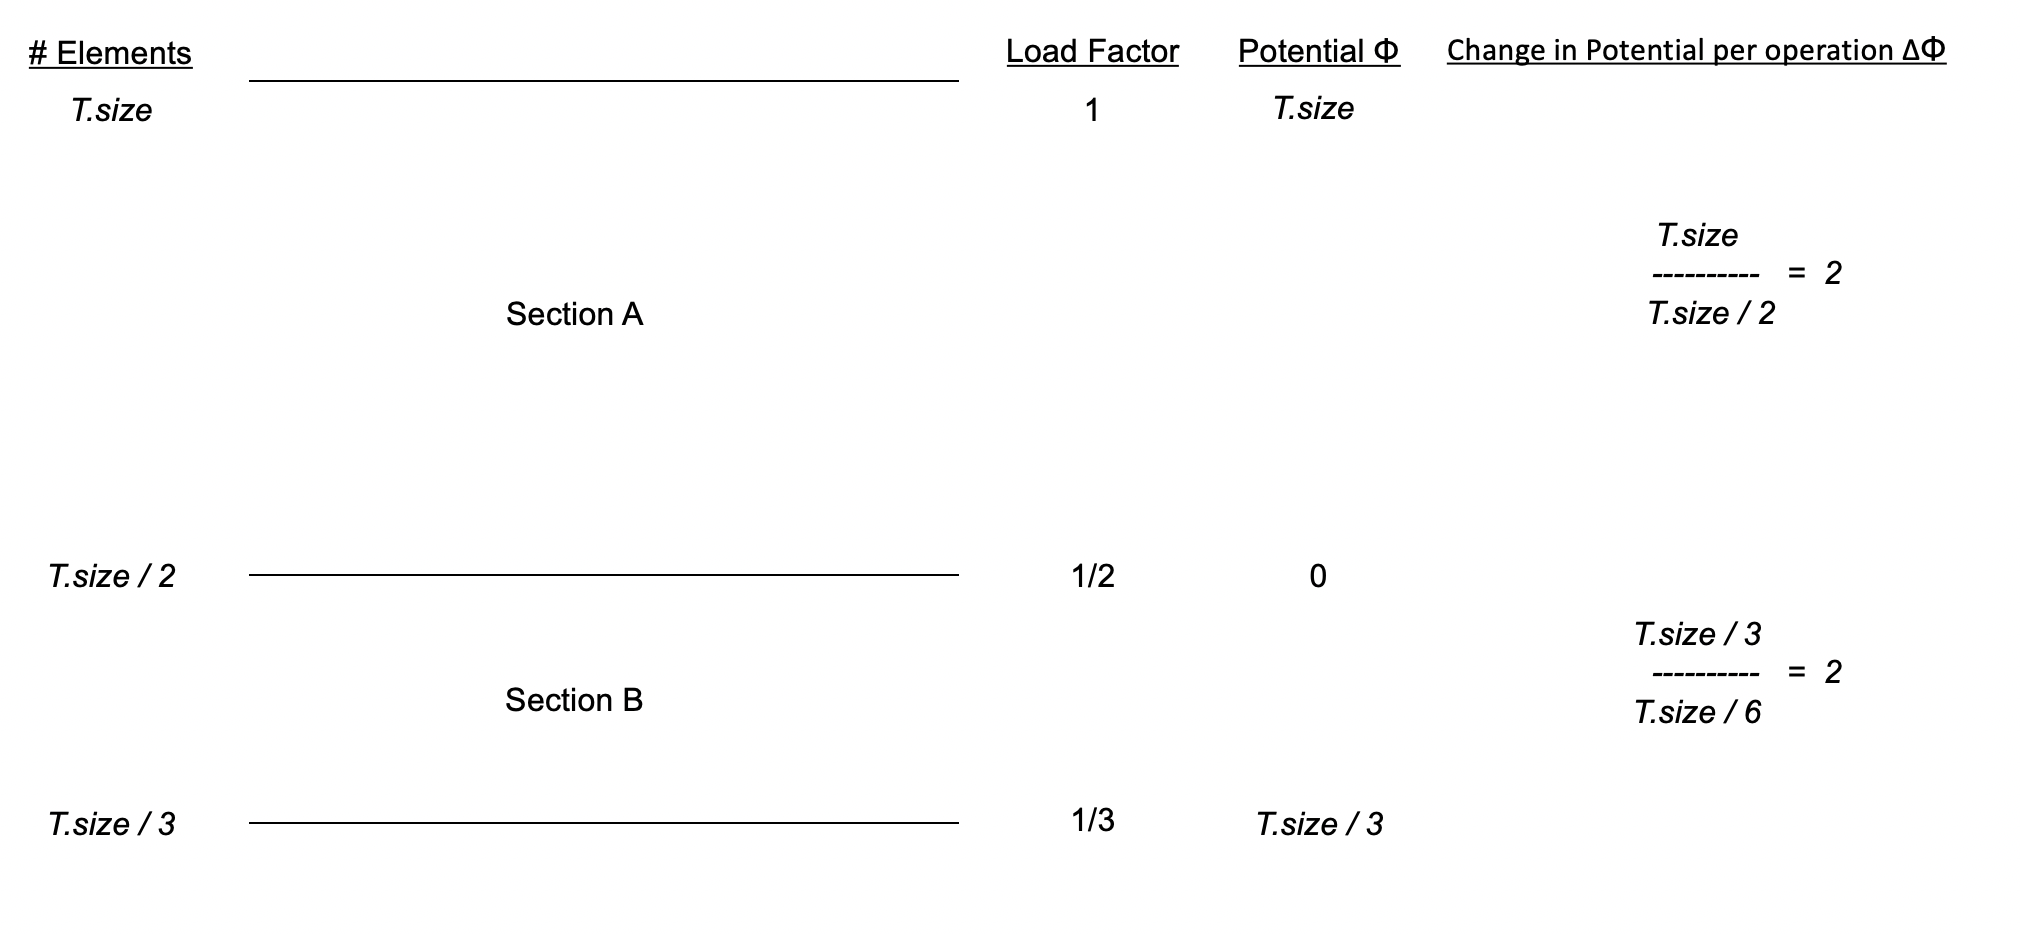
\includegraphics[width=6.5in]{table.png}
\end{figure}

Then, using the method shown in class, let us prove that this implementation yields an amortized cost of \proc{Table-Delete} that is bounded above by a constant. To do so, let us note that we have four cases upon deletion. We define amortized cost as the actual cost plus the change in potential for each case. For each case, let $c_i$ denote the actual cost of the $i$th operation, let $\hat{c_i}$ denote the amortized cost of the $i$th operation, let $\Phi_i$ denote the potential after the the $i$th operation and let $\Phi_{i-1}$ denote the potential before the $i$th operation.

\underline{Case 1:} Deletion without contraction where $\alpha_i \geq 1/2$ (deletion completely within section $A$).

$c_i = 1$ because we are removing a single element without contration.\\
$\Phi_i = T.size$ \\
$\Phi_{i-1} = T.size + 2$ because we have one less element than before and we lose two units of potential on deletion in section $A$

Therefore, $\hat{c_i} = 1 + T.size - (T.size + 2) = 1 - 2 =$ \textbf{-1}.\\

\underline{Case 2:} Deletion without contraction where $1\3 < \alpha_i < 1/2$ (deletion completely within section $B$).

$c_i = 1$ because we are removing a single element without contration.\\
$\Phi_i = T.size + 2$ because we have one less element than before and we gain units of potential on deletion in section $B$ \\
$\Phi_{i-1} = T.size$

Therefore, $\hat{c_i} = 1 + (T.size + 2) - (T.size) = 1 + 2 =$ \textbf{3}.\\

\underline{Case 3:} Deletion without contraction where $\alpha_{i-1} = 1/2$ and $\alpha_i < 1/2$ (deletion straddles $\alpha = 1/2$).

$c_i = 1$ because we are removing a single element without contration.\\
$\Phi_i = 2$ because we gained two units of potential when deleting in section $B$ \\
$\Phi_{i-1} = 0$ because the load factor was 1/2 since we went from section $A$ to $B$

Therefore, $\hat{c_i} = 1 + 2 - 0 =$ \textbf{3}.\\

\underline{Case 4:} Deletion with table contraction.

$c_i = 1 + (\frac{T.size}{3} - 1) = \frac{T.size}{3}$ because we remove one element from $T$ then move $(\frac{T.size}{3} - 1)$ elements into the new table\\
$\Phi_i = 2$ because we removed one element making our size of the new table 1 less than $T.size / 2$\\
$\Phi_{i-1} = T.size/3$ because the load factor was $\alpha = 1/3$ causing us to contract

Therefore, $\hat{c_i} = \frac{T.size}{3} + 2 - \frac{T.size}{3} =$ \textbf{2}.\\

Since we have a constant amortized cost for each possible case, we then know \proc{Table-Delete} is bounded above by a constant.

\newpage

\section{Problem 4-8}
Problem 17-2.
\separateline

\underline{Part A:} To implement \proc{Search} let us perform the following. For some number $n$ where $n$ represents the number of elements in our data structure, we know there exist $k$ sorted arrays $A_0, A_1, ..., A_{k-1}$ where $k = \ceil{\lg{n+1}}$ and the length of each array is $2^i$ for $i = 0,1,...,k-1$. We also know the binary representation of $n$ is $\langle n_{k-1}, n_{k-2}, ..., n_0 \rangle$ and each array is either full or empty depending on whether $n_i = 1$ or 0. Let us denote $x$ as the element we are searching for.

Then, we know if $x$ exists in this data structure, it must exist in a sorted array whose corresponding value of $n$ is 1. Then, the algorithm operates as follows. For each sorted array whose corresponding value of $n$ is 1, we will perform \proc{Binary-Search} on the array if the first element in the array is less than or equal to $x$. Since each array is sorted, we only perform \proc{Binary-Search} on those arrays that are contendors to contain $x$. If the first element is greater than $x$, $x$ cannot exist in the array. Then, if \proc{Binary-Search} finds $x$ in the array, we return \textbf{true}. If \proc{Binary-Search} does not find $x$ in the array, then we will run the algorithm again on the next sorted array whose corresponding value of $n$ is 1. We will continue this process until we return \textbf{true}, or we have exhausted all of our possible arrays in which case we return \textbf{false}. Note that the order in which we try each array will be by size from largest to smallest. Therefore, we wil run \proc{Binary-Search} first on the array of maximal size whose corresonding value of $n$ is 1, followed by the next smallest, etc. By performing \proc{Binary-Search} first on the array of maximal size, we hope to minimize the number of times \proc{Binary-Search} must be called if $x$ is in the data structure.

The worst-case outcome of this algorithm would be if each of the $k$ arrays had a corresponding $n$ value of 1 and we had to search through all $k$ arrays. In this case, we would have $k$ calls to \proc{Binary-Search} where the length of each input is $2^i$ for $i = 0,1,...,k-1$. Since \proc{Binary-Search} runs in $O(\lg{p})$ time for an input of size $p$, each call will then take $O(\lg{2^i})$ time. Since $lg{2^i} = i * \lg{2} = i$, we then have that each call to \proc{Binary-Search} takes $O(i)$ time. Then, using the definition of the arithmetic series, we have:

$\Sigma_{i=0}^{k-1} i = (k-1)(k) / 2 = k^2 - k / 2$.

We therefore have $O(k^2 - k / 2) = O(k^2)$. Since $k = \ceil{\lg{n+1}}$, we then have a worst-case run-time of $O(\lg^2{n})$.\\

\underline{Part B:} To implement \proc{Insert} let us perform the following. Let $x$ denote the element we wish to add to our data structure $T$. Using the notation from above, we then know for $n$ elements in $T$, there exist $k$ sorted arrays $A_0, A_1, ..., A_{k-1}$ where $k = \ceil{\lg(n+1)}$ and the length of each array is $2^i$ for $i = 0,1,...,k-1$. We also know the binary representation of $n$ is $\langle n_{k-1}, n_{k-2}, ..., n_0 \rangle$ and each array is either full or empty depending on whether $n_i = 1$ or 0.

Then, to insert $x$ into $T$, we will first construct a new array and insert $x$ into it. Let $A_x$ denote this array. Let us also note that $A_x$ is sorted since it contains a single element. Since we've added one element to $T$, $T$ will contain $n+1$ elements. Therefore, one 0 in the binary representation of $n$ will flip to a 1 in the binary representation of $n+1$. This bit will be the rightmost 0 in the binary representation of $n$. Let us denote $n_j$ as the rightmost bit will flip from 0 to 1 in the binary representation of $n+1$. Further, we know all bits to the right of $n_j$ will be 0 in the binary representation of $n+1$. Therefore, the binary representation of $n+1$ will simply be the binary representation of $n$ for $n_{k-1}, n_{k-2}...n_{j+1}}$ followed by ${1, n_{j-1}, n_{j-2}, ... n_0}$ where ${n_{j-1}, n_{j-2}, ... n_0}$ are all 0.

Then, in order to insert $x$ into $T$ and have a proper distribution of elements in the proper arrays, we must build up arrays from the array of smallest size at position $n_0$ to position $n_j$. To do so, we will first look at the rightmost array associated with bit $n_0$. Since we know $n_0 = 1$ indicates our data structure contains an array at position $n_0$ and $n_0 = 0$ indicates our data structure does not contains an array at position $n_0$, if $n_0 = 0$, we simply insert $A_x$ into $T$ at position $n_0$ and we are done. In this case, $n_j = n_0$ since the rightmost bit to flip from 0 to 1 is the first bit. Then, $T$ contains one more element, the distribution of arrays maintains the binary representation of $n+1$, and all arrays are sorted.

If $n_0 = 1$, then there exists an array $A_0$ of size 1 at position 0. Then, we will combine $A_0$ with $A_x$, the array we have constructed. To do so, let us call the \proc{Merge} operation from \proc{MergeSort}. This operation will take time $O(p)$ where $p$ represents the number of elements in each array to be combined. In this case, $p=1$ since we are at position 0 in $T$ and an array $A_i$ in $T$ contains $2^i$ elements. Let $A_x$ now denote the combined array of size 2 that results from the call to \proc{Merge}. Using this, let us then move to position $i=1$. If an array $A_1$ exists at position 1 it would contain $2^i = 2^1 = 2$ elements. So, if $n_1 = 0$ no array exists at position 1. Then, since $A_x$ is sorted from the call to \proc{Merge} and it contains 2 elements, we simply insert $A_x$ into position 1. Since we have not changed any subarray to the right of position 1, position 1 now contains an array, and all positions to the right of 1 contain no arrays, we have maintained our binary representation of $n+1$ of $n_{k-1}, n_{k-2}...n_{j+1}, 1, n_{j-1}, n_{j-2}, ... n_0}$ where $n_{j-1}, n_{j-2}, ... n_0}$ are all 0.

If $n_1 = 1$, then there exists an array $A_1$ of size 2 at position 1. Then, we will again combine $A_1$ with $A_x$ using \proc{Merge} and will have a resulting array $A_x$ of size 4. We then will leave position 1 empty and move to position 2. At position 2, we will then repeat the above process of checking if an array exists at position 2, merging if so, or inserting if not. If we iterate through all $k$ arrays and have not found an empty position, then there does not exist a value in the binary representation of $n$ that is 0. In this case, the binary representation of $n+1$ will be one digit larger. The leftmost digit will be 1 and all digits to the right will be 0. Therefore, for the \proc{Insert} method, we will run \proc{Merge} on $A_{k-1}$ and $A_x$ then put the resulting array in a new position $k$, leaving positions $k-1,...0$ empty. Therefore, we will iterate through each position from $i=0$ to $j$, merging subarrays as we go, then inserting our final merged array $A_x$ into position $j$. Since we remove subarrays in positions to the right of $j$, insert an array at position $j$, and leave all arrays to the right of $j$ alone, we will have properly constructed a binary representation of $n+1$.

Let us now analyze the worst-case run time of this implementation. In the worst-case, the binary representation of $n$ contains all 1s, indicating every array in $T$ is full. Then, when inserting a new array into $T$, we must run \proc{Merge} on all $k$ arrays and insert our resulting array in a new position. Since the run-time of \proc{Merge} is $\Theta(m)$ for an input of size $m$, we therefore must sum up the the sizes of each call to \proc{Merge} for arrays 0 to $k-1$. Since each array contains $2^i$ elements for $i=0$ to $k-1$, we then have:

\hspace*{3mm}
\begin{equation}
\begin{split}
\Sigma_{i=0}^{k-1}{2^i} &= 2^{k-1+1} - 1 / 2 - 1\\
                        &= 2^k - 1\\
                        &= 2^{\ceil{lg(n+1)}} - 1\\
                        &\leq 2^{lg(n+1)} - 1\\
                        &= n+1-1\\
                        &= \Theta(n)
\end{split}
\end{equation}

Therefore, we have a total worst-case run-time of $\Theta(n)$.

Let us now analyze the amortized cost of this implementation of \proc{Insert}. To do so, we will use the potential method. We define the potential function $\Phi(T)$ on the data structure $T$ to be $\Phi(T) = nk$ where $n$ represents the number of elements in the table and $k$ represents the number of arrays required to hold those $n$ elements. For an empty data structure $T_0$ from which we start, we have $\Phi(T_0) = 0$. Since $n \geq 0$ and $k \geq 0$ because we cannot have a negative number of elements or a negative number of arrays, we then have $\Phi(T_n) \geq 0$.

Using this, let us construct a table to show the actual cost, change in potential, and amortized cost of the \proc{Insert} operation. Observe that the amortized cost is equal to the actual cost plus the change in potential for each operation.

\begin{table}[H]
\begin{tabular}{l|l|l|l}
operation                   & actual cost & $\Delta \Phi$     & amortized cost \\ \hline
$\proc{Insert}$             & 1                & $(n+1)k - nk = k$                             & $1 + k = 1 + \ceil{\lg(n+1)} = \Theta(\lg{n})$
\end{tabular}
\end{table}

The thought process here is as follows. For \proc{Insert}, the actual cost of this operation is 1 since we must construct a new array and insert $x$ into it. Then, in order to store $n$ elements in the data structure, we must have performed $k$ calls to \proc{Merge}. Since the cost of \proc{Merge} is simply the number of elements being merged together, for each of these $k$ calls to \proc{Merge}, we must have combined $n$ or less elements. In fact, only one of these calls will have merged exactly $n$ elements. $k - 1$ of them will have merged less than $n$ elements. Therefore, by having a potential function of $\Phi(T) = nk$, we pre-pay for the cost of the merges required to construct an additional sub-array.

Given this, we then see that we have an amortized cost of $\Theta(\lg{n})$ for each call to \proc{Insert}.\\


\underline{Part C:} To implement \proc{Delete} let us perform the following. Let us define $x$ as the element we wish to delete from $T$. Let us note that in calling \proc{Delete}, $n$ will be decremented by 1, indicating the binary representation of the number of elements in $T$ will change. Using a thought process similar to that above, the right-most 1 in the binary representation of $n$ will change to a 0, then all digits to the right of this flipped digit will become 1. This is simpy an inverse of the insert case. Therefore, when removing $x$ from $T$, we must also handle moving the contents of subarrays around.

Then, we will first make a call to \proc{Search}, defined above, which will return a reference to the subarray that holds $x$. This will take time $O(\lg^2{n})$. Let us define this array as $A_d$. We will then delete $x$ from $A_d$. Then, we will find the right-most digit in the binary representation of $n$. Let us denote this digit to be at position $j$, indicating the array at position $j$ is $A_j$. We then know the contents of $A_j$ must be dispersed between other pre-existing arrays in $A$ since the binary representation of position $j$ will be going from 1 to 0. In order to do this, we will take the first value in $A_j$ and insert it into $A_d$, the array from which we removed $x$. In order to maintain order in $A_d$, we will call \proc{Merge} on $A_d$ and the element removed from $A_j$. This will take time $O(2^d)$ since $2^d$ elements exist in $A_d$ where $k+1 \geq d \geq 0$.

Then, we will return to $A_j$. With the remaining elements left in $A_j$, we will insert their values into the arrays to the right of $A_j$. Since $j$ was the first position in which the binary representation of $n$ was 1, we know all of the positions to the right of $j$ have a binary representation of 0, indicating no array exists at those locations. So, we will take the first $\frac{2^j}{2}$ elements in $A_j$ and insert them into position $j-1$ (since our ordering is high to low from left to right). We will then take the next $\frac{2^j}{4}$ elements in $A_j$ and insert them into position $j-2$ and so on until we have moved all elements in $A_j$ to arrays in positions to the right of $j$. Since we remove values from $A_j$ in order and each position to the right of $j$ is empty, we do not need to sort or merge any arrays when moving them to new positions. We can also easily prove there exist $2^j - 1$ spots for elements to the right of $j$ to be moved to with the following:

We know there exists $\Sigma_{i=0}^{j-1}{2^i}$ spots at positions to the right of $j$. Using the formula for a geometric series, we then have:

\hspace*{3mm}
\begin{equation}
\begin{split}
\Sigma_{i=0}^{j-1}{2^i} &= 2^{j-1+1} - 1 / 2 - 1\\
                        &= 2^j - 1
\end{split}
\end{equation}

Since $2^j - 1$ elements exist in $A_j$, we have proven enough spaces exist in the positions to the right of $j$ with which to reposition the elements in $j$, excluding that with which we moved to $A_d$, the array from which we removed $x$. Let us note that this holds if $A_d = A_j$. In this case we remove $x$ from $A_j$ so there are $2^j - 1$ elements in $A_j$. We then take the first element in $A_j$ and move it back to $A_j$. Then we disperse the remaining $2^j - 1$ elements in $A_j$ to the positions to the right of $j$.

The run-time of the implementation of this method is $\Theta(n)$ since we call \proc{Merge} on $A_d$ and in the worst case, $A_d$ holds $n$ elements. Dispersing the remaining elements in $A_j$ to the positions to the right of $j$ will take time $\Theta(2^j - 1)$ since we must iterate over all $2^j - 1$ in $A_j$. Since $j$ is at worst the array of maximal size and at worst contains all $n$ elements, this gives us $\Theta(n)$. We therefore have $O(\lg^2{n})$ for the call to \proc{Search} + $\Theta(n) + \Theta(n) = \Theta(n)$ for all sufficiently large $n$.

In a sequence of $n$ \proc{Insert} and \proc{Delete} operations, we then can perform an aggregate analysis. For $n$ operations, we have a total cost of $\Theta(n^2)$ since we must run \proc{Merge} on the $n$ elements at most $n$ times. This gives us a total $\Theta(n^2)$ cost for $n$ operations yielding $\Theta(n)$ per \proc{Delete} operation in a sequence of $n$ \proc{Insert} and \proc{Delete} operations.

\newpage

\section{Who I Worked With}

\textbf{Problem 4-6:} I worked with Kunal Rathi and Emma Rafkin on how to determine the largest half to delete in $O(n)$ time.

\textbf{Problem 4-7:} I worked with Emma Rafkin on determining the potential function and solving all the cases.

\textbf{Problem 4-8:} I worked with Emma Rafkin on determining the proper algorithms for \proc{Insert} and \proc{Delete}

\end{document}
